\documentclass{article}

%usepackages
\usepackage[utf8]{inputenc}
\usepackage{graphicx}
\usepackage[normalem]{ulem}
\usepackage{enumitem}
\usepackage{amsmath}
\usepackage[english]{babel}
\usepackage{amssymb}
\usepackage{amsthm}
\usepackage{todonotes}
\usepackage{hyperref}
\usepackage{pgf,tikz,pgfplots}
\usepackage{mathrsfs}
\usepackage{dirtytalk}
\usepackage[english]{babel}
\usepackage[letterpaper, portrait, margin=1.2in]{geometry}
%\usepackage{fancyhdr}

%new commands
\newcommand{\R}{\mathbb{R}}
\newcommand{\N}{\mathbb{N}}
\newcommand{\Q}{\mathbb{Q}}
\newcommand{\Z}{\mathbb{Z}}
\newcommand{\C}{\mathbb{C}}
\newcommand{\inv}{^{-1}}
\newcommand{\img}{\textmd{Im}\:}
\newcommand{\cok}{\textmd{coker}}
\newcommand{\conv}{\textmd{conv}}
\newcommand{\vertices}{\textmd{vert}}
\newcommand{\st}{\textmd{ s.t. }}
\newcommand{\fracfield}{\textmd{frac}\:}

\newcommand{\celia}[1]{{\color{orange}[[\textbf{Celia says: }#1]]}}
\newcommand{\ad}[1]{{\color{purple}[[\textbf{Ad\'{e}lie: }#1]]}}
\newcommand{\ste}[1]{{\color{green}[[\textbf{Stefania: }#1]]}}

%new theorem environments
%plain
\theoremstyle{plain}
\newtheorem{thm}{Theorem}[section]
\newtheorem{lemma}[thm]{Lemma}
\newtheorem{prop}[thm]{Proposition}
\newtheorem*{ER}{Elder Rule}
%definitions
\theoremstyle{definition}
\newtheorem{definition}{Definition}[section]
\newtheorem{example}{Example}[section]

%remarks
\theoremstyle{remark}
\newtheorem{remark}{Remark}[section]

%pgfplotsset
\pgfplotsset{compat=1.16}

%title
\title{Summary}
\author{Luca Bracone}
\begin{document}
	\maketitle
	\tableofcontents
	\newpage
	\todo{abstract here}
	


	
	\section{Basic Machine Learning}
	\subsection{Neural Networks}
	\begin{definition}[Perceptron]
		A \emph{Perceptron} is a function $ p:\R^n \to \R $ given by 
		\[ p(x_1, \dots , x_n) = g \left( w_0 + \sum_{i=1}^{n} w_i x_i \right)  \]
		Where $ w_1, \dots, w_n \in \R $ are called the \emph{weights} of $p$, $w_0$ is called the \emph{bias}, and $g:\R \to \R $ is any non-linear function called the \emph{activation function}.
		Most of the time we use as activation function \[ g(x)=\frac{e^x}{e^x+1} \] the sigmoid function.
	\end{definition}
%	\begin{minipage}{0.3\textwidth}
%			\includegraphics[width=72px]{figure1.png}
%	\end{minipage}
%\begin{minipage}{0.7\textwidth}
	\begin{definition}[Artificial Neural Network]
		A (forward-feeding) \emph{Artificial Neural Network} (ANN) is a function $T: \R^n \to \R^m$ that can be decomposed as  \[ T= l_k \circ \dots \circ l_1  .\] Where the $l_i : \R^{n_j} \to \R^{n_{j+1}}$ are called \emph{layers} and are just vectors of perceptrons \[ l_i(\vec{x})=(p_{i,1}(\vec{x}),\dots,p_{i,n_{j+1}}(\vec{x})). \]
		In the context of neural networks perceptrons are also called nodes.
	\end{definition}
%\end{minipage}
For some ANN, $T$ and some input $ (x_1,...,x_n) $, we denote $ (y_1,...,y_n) $ the desired output of $ T $. We denote also $ (\hat{y}_1,...,\hat{y}_m) $ the output $T$ actually produced.
\begin{definition}[Loss Function]
	 The \emph{loss} (or sometimes also called \emph{cost})  associated to a neural network $T$ for a given input is a function that measures the `` distance" between the produced and desired output of the network. For most basic applications, the loss is defined as the $l^2$ norm on $\R^n$
	\[\mathcal{L}(W; x)= \sum_{i=1}^{m} ||y_i - \hat{y}_i||_2^2  \]
	Where $W$ is the set of all the weights and biases of every perceptron in $T$.
\end{definition}
\begin{definition}[Empirical Loss]
	For a set of inputs $X=\{(x_1^1,\dots,x_n^1), \dots , (x_1^m,\dots ,x_n^m)\}$, and $T$ an ANN, the \emph{Empirical Loss} is defined as
	\[ J(W)=\frac{1}{|X|} \sum_{\vec{x}\in X} \mathcal{L}(W;x), \]
	the average loss over $X$.
\end{definition}

\subsection{Gradient Descent}
	The output of a neural network depends on the weights and biases of its perceptrons. In order to have the output of the neural network as close as possible to the desired output, one has to find an efficient way to tweak the weights such that the empirical loss becomes as low as possible. To accomplish this task we make repeated use of an algorithm called gradient descent.
	Applying this algorithm involves taking a step in the direction for which the empirical loss is minimised until we reach a stopping condition.  For each weight $w_i$ in $T$, we denote the vector $ \left(\frac{\partial J}{\partial w_i} \right)_{i\in I} $ as $\nabla J$, where $ \frac{\partial J}{\partial w_i} $ with $w_i$ being any weight in $T$, represents how big of a change in $J$ we will obtain by moving $w_i$. The gist of the algorithm revolves around updating the weights with the rule $W \gets W - \eta \nabla J$. Where $\eta$ is a constant that has to be well chosen. If this constant is too small, gradient descent would stop when it meets the slightest uphill. Thus it would miss a better minimum which might be close by. If the constant $\eta$ is too big, gradient descent can only take giant steps and it would diverge to infinity.


	In practice, computing the derivative with respect to some particular weights is not difficult. Consider the following neural network: \\
		\begin{minipage}{0.55\linewidth}
        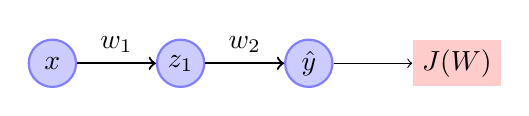
\begin{tikzpicture}[perceptron/.style={circle, draw=blue!50,fill=blue!20,thick, inner sep=0mm, minimum size= 6mm},
        scalar/.style={rectangle, fill=red!20}]
        \node (input) [perceptron] {$x$};
        \node (hidden) [perceptron, right= of input] {$z_1$}; 
        \node (output) [perceptron, right= of hidden] {$\hat{y}$};
        \node (loss) [scalar, right = of output] {$J(W)$};
        \draw[->, thick] (input) to node[auto] {$w_1$} (hidden);
        \draw[->, thick] (hidden) to node[above] {$w_2$} (output);
        \draw[->] (output) to (loss);
		\end{tikzpicture}
		\end{minipage}
	\begin{minipage}{0.4\linewidth}
	    The gradient descent can be computed with an application of the chain rule:
		\begin{align*}
		\frac{\partial J}{\partial w_2} &=\frac{\partial J}{\partial \hat{y}} \frac{\partial \hat{y}}{\partial w_2} \\
		\frac{\partial J}{\partial w_1} &= \frac{\partial J}{\partial \hat{y}}\frac{\partial \hat{y}}{\partial z_1}\frac{\partial z_1}{\partial w_1}
		\end{align*}
	\end{minipage}

	Since calculating $\nabla J$ is computationally intensive, one can consider to take a random subset of the data, and applying gradient descent to it instead. The convergence is going to be more erratic, depending on the size of the subset chosen.
	\subsection{Overfitting}
	When training our neural network, it might happen that it essentially \say{learns the data set by heart} making it unable to properly tackle on never seen before data points. There are a few methods to avoid such a problem:
		\begin{figure}[ht!]
		\centering
		\includegraphics{overfitting.png}
		\caption[image of overfitting]{A parabola+noise is being misunderstood as a complicated winding line \protect \footnotemark}
		\end{figure}
		\footnotetext{Courtesy of wikimedia foundation \href{https://commons.wikimedia.org/wiki/File:Overfitting.svg}{https://commons.wikimedia.org/wiki/File:Overfitting.svg}}
		
	\emph{Dropout} involves randomly setting some nodes to zero during training. This makes the network not rely too much on some path.
	\emph{early stopping} is the process by which after each application of gradient descent, one tests the network. If it performs worse than it did previously, stop the training process.	
	\ste{This section needs to be reviewed in the future}
	\section{Simplicial Complexes}
	\begin{definition}[Convex Hull]
	Let $ u_0,...,u_k \in \R^n $ their \emph{convex hull} is defined as
	  \begin{equation} 
	  \label{conv-hull}
	  \conv \{u_0,...,u_k\} = \left\{ x= \sum_{i=0}^{n} \lambda_i u_i \ :    \sum_{i=0}^{n} \lambda_i = 1; \ \lambda_i > 0 \ \forall i \right\} 
	  \end{equation}
	\end{definition}
	
	\begin{definition}[Affinitely Independent, $k$-simplex]
		Let $u_0,...,u_k \in \R^n$ . They are said to be \emph{affinitely independent }if any point in their convex hull, when written as in ~\eqref{conv-hull} the coefficients $\lambda_i$ are unique.
		In that case instead of convex hull, we speak of \emph{$k$-simplex}. The \emph{dimension} of a $k$-simplex is $k$.
	\end{definition}
	
	\begin{definition} [Faces and Co-faces]
		Let $ \{u_{i_0},...,u_{i_m} \}$ be a subset of $\{u_0,...,u_k\} $. In this case, we say that $ \tau = \conv\{u_{i_1},...,u_{i_m}\} $ is a \emph{face} of $ \sigma = \conv\{u_1,..,u_k\} $ which we write $ \tau < \sigma $. Equivalently, $ \sigma $ is said to be a \emph{co-face} of $ \tau $.
	\end{definition}
	
	\begin{definition}[Simplicial Complex]
		A \emph{simplicial complex} $K$ is a collection of simplices such that:
		\begin{enumerate}[label=(S\arabic*)]
			\item $ \forall \sigma \in K, \ \tau < \sigma \implies \tau \in K $. 
			\item $ \forall \sigma,\tau \in K, \ \sigma \cap \tau $ is either empty or a face.
		\end{enumerate}
	The \emph{dimension} of $K$ is $ \dim K = \max_{\sigma \in K} \dim \sigma $.
	The \emph{underlying space} of $K$, $|K|$ is the topological space $ \bigcup_{\sigma \in K} \sigma $ with the subspace topology.
	\end{definition}
\todo{simple examples of complexes}
\begin{definition}[Triangulation]
	Let $X$ be a topological space and $K$ a simplicial complex, if there exists a homeomorphism $ \phi : X \to |K| $ we say that $X$ is triangulable. In that case the couple $ (K,\phi) $ is called a triangulation of $X$
\end{definition}

	\begin{definition}[sub-complex]
		A subset $L \subseteq K$ is a \emph{sub-complex} of K if it is itself a simplicial complex. It is called full if it contains all vertices of $K$.
	\end{definition}
	
	\begin{example}[Skeleton]
		The \emph{$j$-skeleton} of a simplicial complex $K$ is $K^{(j)}= \{ \sigma \in K \st \dim\sigma \leq j \} \subseteq K $. In particular the 0-skeleton is denoted by $\vertices(K)$ and it consists of the vertices of $K$
	\end{example}
	
	\begin{definition}[Star and Link]
		Let $K$ be a simplicial complex and pick $ \sigma \in K $. Its \emph{star}, is the set \[ st (\sigma) = \{ \tau \in K \st \tau < \sigma \} \].
		Let $\overline{st} (\sigma)$ be the smallest sub-complex that contains $st(\sigma)$, we call it the \emph{closed star} of $\sigma$. \\
		Similarly, the \emph{link} of a simplex \[ lk (\sigma) = \{ \tau \in \overline{st}\sigma \st \tau \cap \sigma = \emptyset \} \] the set of simplices in the closed star that don't touch $\sigma$
	\end{definition}
	\begin{remark}
        Note that the star of a $k$-simplex $\sigma$ is not necessarily a sub-complex of $K$ because it's not closed under taking faces. This motivates the definition for the closed star $ \overline{st} (\sigma) $.
	\end{remark}
	\begin{definition}[Simplicial Maps and Homeomorphisms]
		Let $K$, $L$ be two simplicial complexes and $ \phi: \vertices K \to \vertices L $ a map such that vertices of every simplex in $K$ gets mapped to a vertex of a simplex in $L$, in that case $\phi$ is called a \emph{vertex map}.The map $f: |K| \to |L|$ defined by $ \sum_{i=0}^n \lambda_i u_i \mapsto \sum_{i=0}^n \lambda_i \phi(u_i) $ is called a \emph{simplicial map}. If $ \phi $ is bijective and $ \phi\inv $ is also a vertex map, we call it instead a \emph{simplicial homeomorphism}.
	\end{definition}

	\section{Simplicial Homology}
	\begin{definition}[$p$-chain]
		Let $K$ be a simplicial complex. A \emph{$ p $-chains} is a formal sum of $p$-simplices of $K$ over a field $F$ \[ c = \sum_{i=1}^{n} a_i \sigma_i. \] Where $\sigma_i \in K$ and $a_i \in F$
	\end{definition}
	For the time being, the field in question is $F = \mathbb{F}_2 $. Component-wise addition: $ c + d = \sum_{i=1}^n (c_i + d_i) \sigma_i $ makes the set of $p$-chains into a commutative group which we note as $ (C_p, +) $.
\begin{definition}[Boundary]
	The \emph{boundary} of a $ p $-simplex is a map $ \partial_p : C_p \to C_{p-1} $ which for a $p$-simplex returns the sum of the $ (p-1) $-faces: \[ \partial_p \sigma = \sum_{j=1}^n [u_1, \dots , \hat{u}_j , \dots , u_p] \]
	where $[ u_1 \dots u_p ]$ is the $p$-simplex given by the convex hull of $\{u_1, \dots , u_p\}$ and $\hat{u}_j$ means we omit the $j$-th term from that notation.
	This definition extends by linearity to the $p$-chains: \[ \partial_p c = \sum_{i=1}^{n} a_i \ \partial_p\sigma_i  \]
\end{definition}

It turns out that $ \partial_p : C_p \to C_{p-1} $ is a group homomorphism. For a simplicial complex $K$ we define its chain complex:
\[\mathcal{C}_K: \ \dots \longrightarrow C_p \stackrel{\partial_p}{\longrightarrow} C_{p-1} \stackrel{\partial_{p-1}}{\longrightarrow} \dots \stackrel{\partial_1}{\longrightarrow} C_0 \longrightarrow 0 \]

\begin{thm}[Fundamental Lemma of Homology]
	For all $p$ and $d \in C_{p+1}$, we have $ \partial_{p} \partial_{p+1} d = 0$
\end{thm}

Whenever we have an interesting homomorphism it is natural to want to know more about its kernel and image, in this case they have special names:

\begin{definition}[$p$-boundaries and $p$-cycles]
	The \emph{$p$-cycles} are the elements which belong to the kernel: \[ \ker\partial_{p} = \{ c \in C_p : \partial_p c = 0 \} := Z_p \]
	The \emph{$p$-boundaries} are the elements which are given as the boundary of a $(p+1)$-chain \[ \img\partial_{p+1} = \{ c \in C_p : \exists d \in C_{p+1} , \ c=\partial_{p+1} d \} := B_p \]
\end{definition}

\begin{remark}
Whenever it is clear, we favour the notation $\partial$ over $\partial_p$, omitting the $p$. 
\end{remark}
\begin{remark}
Furthermore, note that if $ c \in B_p $ then $ \partial c = \partial \partial d = 0 $. Thus we notice that $ B_p \subseteq Z_p $. But in general $ B_p \neq Z_p $. %In particular, we are interested in the $p$-cycles that are not $p$-boundaries.
The difference between $p$-cycles and $p$-boundaries is what motivates the definition of homology groups.
\end{remark}

\begin{definition}[Homology Groups and Betti numbers]
	For a complex $K$ its $p$-th \emph{homology group} is the quotient $H_p = Z_p/B_p $.\\
	The $p$-th \emph{Betti number} is $ \beta_p $ the number of generators of $H_p$.
\end{definition} 

\begin{example}
Consider the simplex drawn in picture ~\ref{fig:example1} on page ~\pageref{fig:example1}, it consists of the union of two tetrahedrons except that for the upper one we removed its volume as well as all its faces, while for the bottom one we remove its volume.
Let’s calculate its homology groups. \\ First notice that $H_0 = \langle [v] \rangle $ where $[v]$ is the equivalence class of any $0$-chain whose sum is comprised of a single vertex. Indeed, for $\partial: C_0 \to 0$ the kernel is the whole group $C_0$. On the other hand, since $K$ has one connected component, for any two vertices $u,w$ there is a $1$-chain (which can be thought of as a path between $u$ and $w$) such that its boundary is $u+w$. Thus, $B_0$ is comprised of the $0$-chains that have an even number of summands. Therefore $H_0$ contains two classes: the $0$-chains that have are the sum of an even number of vertices which are equivalent to the zero $0$-chain, and the $0$-chains that are the sum of an odd number of vertices which are equivalent to the $0$-chains with only one summand. The choice of $v$ for the representative does not matter because $K$ has one connected component, for any other two vertices $x,y$ in $H_0$ we may write 
\[v = v+0 = v + \partial p_{x,y} = v + x + y = \partial p_{v,x} + y = y.  \] Where $p_{x,y}$ denotes a $1$-chain whose boundary is $x+y$. \\
Now for $H_1$, to alleviate the notation we write $e_{i,j}$ for the $1$-simplex $(v_iv_j)$. We notice that the 1-chain made up of the 1-simplices that form a face of one of the “empty triangles” namely, \[ e_{1,4} + e_{4,3} + e_{3,1},\ e_{5,4} + e_{4,3} + e_{3,5},\ e_{1,5} + e_{5,3} + e_{3,1},\ e_{1,4} + e_{4,5} + e_{5,1} \] are cycles, but that they are not the boundary of any 2-chain. Thus for each empty face, we have a generator of $H_1$. There are no other generators because for any other $1$-cycle we may sum it with a certain combination of the following $1$-chains \[ e_{1,2} + e_{2,3} + e_{3,1}, e_{5,2} + e_{2,3} + e_{3,5}, e_{1,5} + e_{5,3} + e_{3,1}, e_{1,2} + e_{2,5} + e_{5,1} \]  in order to find one that we have already found. For example
\[ e_{1,2} + e_{2,3} + e_{3,4} + e_{4,1} \ + \ e_{1,2} + e_{2,3} + e_{3,1} = e_{1,4} + e_{4,3} + e_{3,1} .\] So, $H_1$ is the free commutative group generated by $\{f,g,h\}$ where $f,g,h$ are the 1-chains that each correspond to one of the empty triangles in the upper tetrahedron. \\
Lastly, for $H_2$ there is only one 2-cycle that is not a 2-boundary, which is the “shell” of the bottom tetrahedron, because we specifically made it empty. Therefore, $H_2$ is the free group generated by the 2-chain that corresponds to that shell. If that volume were to be full, $H_2$ would instead be trivial.\\
The group $H_3$ is trivial because there are no 3-chains. \\
We see that the Betti numbers are $\beta_0 = 1$, $\beta_1 = 3$, $\beta_2 = 1$, $\beta_n = 0$ for all $n \geq 3$
In general, $\beta_0$ can be thought of as the number of connected components, $\beta_1$ as the number of holes, $\beta_2$ the number of empty volumes, and  $\beta_n$ as the number of \say{$n$-dimensional holes}.
\end{example}

\begin{figure}[ht!]
\begin{center}
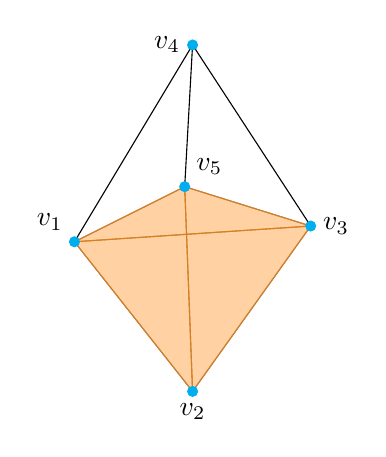
\begin{tikzpicture}[node distance = 1pt]

\coordinate (v2) at (0,-3.5) {};
\node[below= of v2] {$v_2$};
\coordinate (v1) at (-1.5,-1.6) {};
\node[above left= of v1] {$v_1$};
\coordinate (v3) at (1.5,-1.4) {};
\node[right= of v3] {$v_3$};
\coordinate (v4) at (0,0.9) {};
\node[left= of v4] {$v_4$};
\coordinate (v5) at (-0.1,-0.9) {};
\node[above right= of v5] {$v_5$};

\draw[brown] (v1) -- (v2) -- (v3) -- cycle;
\draw[brown] (v5) -- (v2) -- (v3) -- cycle;
\draw[brown] (v1) -- (v5) -- (v3) -- cycle;
\draw[brown] (v1) -- (v2) -- (v5) -- cycle;

\fill[orange, opacity=0.2] (v1) -- (v2) -- (v3) -- cycle;
\fill[orange, opacity=0.2] (v5) -- (v2) -- (v3) -- cycle;
\fill[orange, opacity=0.2] (v1) -- (v5) -- (v3) -- cycle;
\fill[orange, opacity=0.2] (v1) -- (v2) -- (v5) -- cycle;
\draw (v1) -- (v4) -- (v3);
\draw (v4) -- (v5);
\foreach \n in {1,...,5}
    \fill[cyan] (v\n) circle (2pt);
\end{tikzpicture}
\caption{An example of a simplicial complex embedded in $\R^3$}
\label{fig:example1}
\end{center}
\end{figure}


\begin{definition}[Induced Map]
	Consider two complexes $K$, $L$ and a simplicial map $ f: K \to L $. We have a way to transform $f$ into a map $ f_\sharp: C_p(K) \to C_p(L) $, in this way 
	\[ c = \sum_{i=1}^n a_i \sigma_i \ \mapsto \ \sum_{i=1}^{??} a_i \tau_i  \]
	Where $ \tau_i = f(\sigma_i) $ if it has dimension $p$ or $ \tau_i =0 $ otherwise. We call $f_\sharp$ the \emph{induced map} of $f$.
\end{definition}

\section{Persistent Homology}

\begin{definition}[Level Sets]
For a topological space $X$ and a map $f:X\to \R$, its \emph{level sets} are $ X_a=\{ x \in X \st f(x) \leq a\} $
\end{definition}

Suppose $f$ is continuous. For each $X_a$ we consider its connected components, we can imagine a picture where on the vertical axis we have the real number line and horizontally we plot a point for each connected component of $X_a$. This effectively gives a graph, and if $f$ is monotone, a tree. This is called the \emph{merge tree} of $X$ under $f$. Its vertices are located at times where two components merge, and the edges represent the existence of a component over time. \\
We would like to attach an identity to these components, so we use the following rule:
\begin{ER}
When two components merge, we keep the oldest one. The younger is said to die or to merge into the older one.
\end{ER}

Using the level sets, we define an increasing chain of sub-complexes. Indeed, if $f:K \to \R$ is monotone (that is whenever $\sigma < \tau$, $f(\sigma) < f(\tau)$) and continuous, the level sets $f\inv(-\infty, a] = K(a)$ are sub-complexes of $K$. \\
We now write $K_i$ instead of $K(a_i)$.
\begin{definition}[Filtration]
Let $K$ be a complex. The sequence of inclusions,
\[ \emptyset = K_0 \subseteq K_1 \subseteq \dots \subseteq K_{n-1} \subseteq K_n = K \] is called a \emph{filtration} of $f$.
\end{definition}

From a filtration we obtain a sequence of Homology groups 
\[ H_p(K_0) \rightarrow \dots \rightarrow H_p(K_n) \] where the arrows are the homomorphisms induced by the inclusion maps.

\begin{definition}[Persistent Homology Groups and Persistent Betti Numbers]
Considering the above chain of homology groups, the $p$-th persistent homology groups are defined as $H_p^{i,j} := \img f_p^{i,j}$. Where $f_p^{i,j}: H_p(K_i) \hookrightarrow H_p(K_j)$ is the homomorphism induced by the inclusion. \\
The $p$-th persistent \emph{Betti Number}, $\beta_p^{i,j}$ is the number of generators of $H_p^{i,j}$
\end{definition}
\begin{remark}
Under this definition, $H_p^{i,i}$ is the $p$-th homology group of $K_i$
\end{remark}
\newpage %this is needed only if "example" and the tikz image keep showing on different pages
\begin{example}\ \\
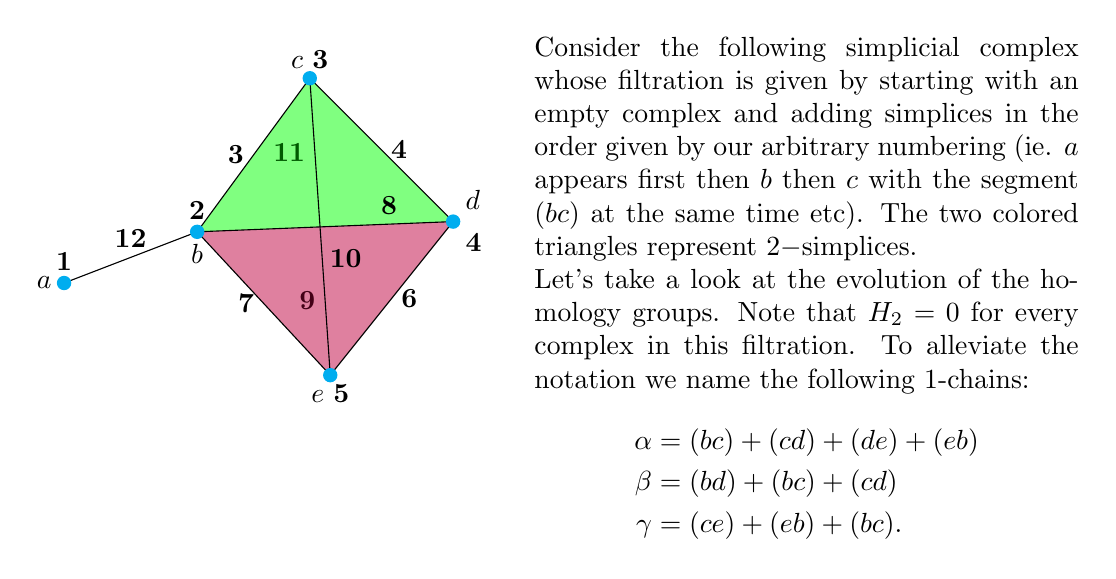
\begin{tikzpicture}[scale=1.3]

\coordinate (a) at (0.5,0.5);
\node[left=1pt of a] {$a$};
\node[above=1pt of a] {\textbf{1}};
\coordinate (b) at (1.8,1);
\node[below=1pt of b] {$b$};
\node[above=1pt of b] {\textbf{2}};
\coordinate[label=above:{$c$ \textbf{3}}] (c) at (2.9,2.5);
\coordinate (d) at (4.3,1.1) ;
\node[above right=.5mm of d] {$d$};
\node[below right=.5mm of d] {\textbf{4}};
\coordinate[label=below:{$e$ \textbf{5}}] (e) at (3.1,-0.4);

\fill[color=green!50] (b) -- (c) -- (d) -- cycle;
\fill[color=purple!50] (b) -- (d) -- (e) -- cycle;

\draw (a) -- node[above] {\textbf{12}} (b) -- node[left] {\textbf{3}} (c) -- node[right] {\textbf{4}}  (d) -- node[right]{\textbf{6}} (e) -- node[left] {\textbf{7}} (b) -- node[auto, near end] {\textbf{8}} (d);
\draw (c) -- node[left, near start, color=black!65!green] {\textbf{11}} node[left, near end, color=black!65!purple](eleven) {\textbf{9}} node[below=.4cm of eleven, right] {\textbf{10}} (e);

\foreach \point in {a,b,c,d,e}
    \fill[cyan] (\point) circle (2pt);

\node [below right, text width=.57\textwidth,align=justify] at (5,3) {Consider the following simplicial complex whose filtration is given by starting with an empty complex and adding simplices in the order given by our arbitrary numbering (ie. $a$ appears first then $b$ then $c$ with the segment $(bc)$ at the same time etc). The two colored triangles represent $2-$simplices. \\ Let's take a look at the evolution of the homology groups. Note that $H_2=0$ for every complex in this filtration. To alleviate the notation we name the following 1-chains: 
\begin{align*}
    \alpha &= (bc)+(cd)+(de)+(eb) \\
    \beta  &= (bd)+(bc)+(cd) \\
    \gamma &= (ce)+(eb)+(bc).
\end{align*}};
\end{tikzpicture}
\\
We calculate the following homologies:
\begin{center}
\begin{tabular}{|l|l|l|l|l|l|}
    \hline
     \textbf{(1)}&\textbf{(2)}&\textbf{(3)}&\textbf{(4)}&\textbf{(5)}&\textbf{(6)}  \\
     $ H_0=\langle a \rangle $ & 
     $ H_0=\langle a,b \rangle $ &
     $ H_0=\langle a,b \rangle $ &
     $ H_0=\langle a,b \rangle $ &
     $ H_0=\langle a,b,e \rangle $ &
     $ H_0=\langle a,b \rangle $ \\
     $H_1 = 0$ &
     $H_1 = 0$ &
     $H_1 = 0$ &
     $H_1 = 0$ &
     $H_1 = 0$ &
     $H_1 = 0$ \\
    \hline
     \textbf{(7)}&\textbf{(8)}&\textbf{(9)}&\textbf{(10)}&\textbf{(11)}&\textbf{(12)}\\
     $ H_0=\langle a,b \rangle $ &
     $ H_0=\langle a,b \rangle $ &
     $ H_0=\langle a,b \rangle $ &
     $ H_0=\langle a,b \rangle $ &
     $ H_0=\langle a,b \rangle $ &
     $ H_0=\langle a \rangle $ \\
     $H_1=\langle \alpha \rangle$ &
     $H_1=\langle \alpha,\beta  \rangle$ &
     $H_1=\langle \alpha \rangle$ &
     $H_1=\langle \alpha, \gamma \rangle$ &
     $H_1=\langle \gamma \rangle$ &
     $H_1=\langle \gamma \rangle$ \\
    \hline
\end{tabular}
\end{center}
(If the reader wants to compute the same table, we recommend he or she draws a picture for each complex in the filtration).\\
Notice how in step 12, it is $a$ that is kept, rather than $b$. This is the elder rule in action.
Notice how in step 8, we might think that two new generators were added, one for each empty triangle, but in reality only $\beta$ is added. The other one is a sum of the generators who are already present:
\[(be)+(ed)+(db)=(bc)+(cd)+(de)+(eb)+(bc)+(cd)+(bd)= \alpha + \beta  \]
Likewise in step 10 one might think that a generator is added for each of the two empty triangles created but only one is really added. The other one is a sum of the two:
\[ (ed)+(dc)+(ce) = (ce)+(eb)+(bc)+(bc)+(cd)+(de)+(eb) = \gamma + \alpha \]

\end{example}

The classes of $H_p(K_i)$ represent $p$-dimensional holes \say{when viewing $K$ at a certain resolution}. It is then apparent that if a certain $p$-dimensional hole is visible for various resolutions, then it somehow exists or represents an important feature in the \say{real complex}. To make this idea clearer we introduce the following vocabulary.

\begin{definition}
Let $\gamma \in H_p^{i,i} $. If $\gamma \notin H_p^{i-1,i}$ we say that $\gamma$ is \emph{born at $K_i$}. \\
Furthermore if $f_p^{i,j-1}(\gamma) \notin H_p^{i-1,j-1}$ and $f_p^{i,j} \in H_p^{i-1,j}$ then we say that $\gamma$ \emph{dies entering $K_j$} \\
The \emph{persistence} of $\gamma$ is the number $a_j-a_i$
\end{definition}

Let $\mu_p^{i,j}$ be the number of classes born at $K_i$ and dying at $K_j$. In other words 
\[ \mu_p^{i,j} = \left( \beta_p^{i,j-1} - \beta_p^{i,j} \right) - \left( \beta_p^{i-1,j-1} - \beta_p^{i-1,j}  \right) \]
indeed, the first difference counts the classes that are born at or before $K_i$ and that die entering $K_j$ while the other counts those that are born strictly before $K_i$ and die entering $K_j$.

We now look for a way to visualise all the gained information. For that, we look to \emph{Persistence Diagrams}. For each class that appears, draw a point at coordinates $(a_i,a_j)$ with multiplicity $\mu_p{i,j}$. Where $a_i$ is when it was born and $a_j$ when it died.

\begin{example}
Consider the persistence diagram illustrated in figure ~\ref{fig:torus-rips-persisntence} in page ~\pageref{fig:torus-rips-persisntence} computed using Vietoris-Rips filtration. It represents the persistence classes of a point cloud in the shape of a torus. The points that stick out from the diagonal are the classes whose persistence is greater, and thus most worthy of attention. We can see that the fact there is only one connected component is quickly detected. We also see that the filtration identifies four classes of 1-dimensional holes, two disappear quickly and the other two (which are almost stacked on top of each other) are the loops on the torus we already are familiar with. Finally, the 2-dimensional hole, i.e the \say{volume} of the torus, is clearly identified.
\end{example}

\begin{figure}[ht]
    \centering
    \includegraphics[scale=.5]{torus-rips-persistence.png}
    \caption{Persistence diagram of a torus}
    \label{fig:torus-rips-persisntence}
\end{figure}

\section{Cubical Homology}

\begin{definition}[Elementary Interval]
Let $z \in \Z$ an integer. \emph{Elementary intervals} are subsets of $\R$ the form $ [z,z+1] $ or $ [z]= \{z\} $. In the latter case, it is said to be degenerate.  
\end{definition}

\begin{definition}[Elementary Cube]
An \emph{elementary cube} is a Cartesian product of elementary intervals, $ \prod_{i\in J} I_i $. The set of all elementary cubes is denoted $K$, and $K^d$ is the set of all elementary cubes for which $|J| = d$.
\end{definition}

\begin{definition}[Embedding Number, Component and Dimension]
For an elementary cube $Q= I_1 \times \dots \times I_d \subset \R^d$, its \emph{embedding number}, $emb(Q)$ is $d$. Its $i$-th component is $I_i$ and its dimension, $dim(Q)$ is the number of non-degenerate components. \\
The set of elementary cubes whose dimension is $k$ is denoted $K_k$ and $K_k^d := K_k \cap K^d$
\end{definition}

\begin{prop}
Let $Q\in K_k^d$ and $P\in K_{k'}^{d'}$, then $Q \times P \in K_{k+k'}^{d+d'}$
\end{prop}

\begin{definition}[Faces]
Let $Q,P \in K$. If $Q\subseteq P$, we say that $Q$ is a face of $P$, which we note as $Q \preceq P$, and $Q \prec P$ if it is a proper inclusion. Also, $Q$ is said to be a primary face of $P$ if $dim(Q) = dim(P) - 1$.
\end{definition}

\begin{definition}[Cubical Set]
A set $X$ is said to be cubical if $X= \bigcup_{i\in J} Q_i $ where $Q_i \in K \ \forall i $. We then have the following sets: $K(X) := \{ Q \in K | Q \subset X \}$ and $K_k(X) := K_k \cap K(X)$
\end{definition}

\begin{definition}[k-chain]
For a finite collection of elementary $k$-dimensional cubes $\{ Q_1, \dots , Q_m \} \subset K_k^d$, a $k$-chain is a formal sum over a field $F$, $c=\sum_{i=1}^n a_i Q_i$. The set of $k$-chains is denoted $C_k^d$.
\end{definition}

\begin{remark}
Point-wise addition: \[ \sum_{i=1}^n a_i Q_i + \sum_{i=1}^n b_i Q_i = \sum_{i=1}^n (a_i+b_i) Q_i \] makes $C_k^d$ into a group.
\end{remark}

\begin{prop}
Let $Q \in K^d$ then there exist unique $I \in K^1$ and $P \in K^{d-1}$ such that $Q= I \times P$
\end{prop}

\begin{definition}[Boundary]
Let $\partial_k : C_k^d \to C_{k-1}^d$ be the map defined by induction: 
\begin{itemize}
    \item If $d=1$, $\partial_k Q =
    \begin{cases}
    0 \ \textmd{if} \ Q=[z] \\
    [z+1] - [z] \ \textmd{if} \ Q=[z,z+1]
    \end{cases}$
    \item if $d>1$, $\partial_k Q = \partial_{k_1} I \times P + (-1)^{k_1} I \times \partial_{k_2}P $. Where $k_1$ and $k_2$ are the dimensions of $I$ and $P$  
\end{itemize}
\end{definition}

\begin{remark}
Using linearity to define the boundary on any $k$-chain, we obtain that the boundary is a homomorphism.
\end{remark}

\begin{prop}\ Let $c,d$ be k-chains. Then, \[ \partial(c \times d) = \partial c \times d + (-1)^{dim c} c \times \partial d \]
\end{prop}

\begin{prop}
Let $Q_1, \dots , Q_m$ be elementary cubes. Then, 
\[ \partial(Q_1 \times \dots \times Q_m) = \sum_{j=1}^m (-1)^{\sum_{i=1}^{j-1} dim Q_i} Q_1 \times \dots \times Q_{j-1} \times \partial Q_j \times Q_{j+1} \times \dots \times Q_m \]
\end{prop}

\begin{prop}
Let $Q= I_1 \times \dots \times I_d$ be an elementary cube such that $I_j = [k_j, k_j+1]$. Let 
\begin{align*}
Q^+_j &= I_1 \times \dots \times I_{j-1} \times [k_j] \times I_{j+1} \times \dots \times I_m \\
Q^-_j &= I_1 \times \dots \times I_{j-1} \times [k_j+1] \times I_{j+1} \times \dots \times I_m 
\end{align*}
Then, \[ \partial Q = \sum_{j=1}^n (-1)^{j-1} (Q^+_j - Q^-_j) \]
\end{prop}

\begin{example}
Let $Q=[l,l+1] \times [k,k+1]$ then 
\begin{align*}
    \partial_2 Q &= \partial_1 [l,l+1] \times [k,k+1] + (-1)^{dim [l,l+1]} [l,l+1] \times \partial_1 [k,k+1] \\ 
    &= ([l+1] - [l]) \times [k,k+1] - [l,l+1] \times ([k+1] - [k]) \\
    &= [l+1] \times [k,k+1] - [l] \times [k,k+1] - [l,l+1] \times [k+1] + [l,l+1] \times [k]
\end{align*}
\end{example}

\begin{lemma}
For any $k\in \N$ and $Q \in C_{k+1}$, $\partial_k \partial_{k+1} Q = 0$
\end{lemma}

When it is clear, we write $\partial$ instead of $\partial_k$

\begin{prop}
For any $c\in C^d_k$, $\partial c \subset c$. Moreover, $\partial c$ is contained in the $(k-1)$-skeleton of $c$ that is the union of the $(k-1)$-dimensional faces of $c$.
\end{prop}

\begin{definition}
The sets $C_k(X) = \left\{ \sum_{i\in J} a_i Q_i | a_i \in F, Q_i \in K_k(X) \right\}$ are the $k$-chains of $X$. \\
The cubical chain complex of $X$ is the following sequence of chain groups and boundary operations:
\[ \mathcal{C}(X): \ \dots \stackrel{\partial}{\longrightarrow} C_k(X) \stackrel{\partial}{\longrightarrow} \dots \stackrel{\partial}{\longrightarrow} C_1(X) \stackrel{\partial}{\longrightarrow} C_0(X) \]
\end{definition}

\begin{definition}
The elements belonging to the kernel of the $k$-boundary morphism $Z_k(X) := \ker\partial_k$ are called $k$-cycles, while those belonging to the image of the $(k+1)$-boundary $B_k(X) = \img \partial_{k+1}$ are called $k$-boundaries.
\end{definition}

\begin{definition}[Cubical Homology Groups]
The $k$-th cubical homology group is the quotient $ H_k(X)=Z_k(X)/B_k(X) $
\end{definition}

Now that we have cubical homology groups we can start calculating persistence diagrams of images. We begin by only considering gray scale images.
\begin{definition}
An \emph{Image} is a function $f:\R^2 \to \R$ such that:
\begin{enumerate}
    \item If $p \in [l,l+1] \times [k,k+1]$ and $f(p)=\alpha$ then $\forall q \in [l,l+1] \times [k,k+1], f(q)=\alpha$
    \item There exists $k_{max},l_{max} \in \Z$ such that if $|k|>k_{max}$ or $|l|>l_{max}$ then \[\forall p \in [l,l+1] \times [k,k+1], f(p) = 0\]
\end{enumerate}
\end{definition}
In other words $f$ is a pixel wise coloring of a finite rectangular area of $\R^2$.
To obtain a filtration, we consider the sublevel sets of $f$:
\[ X_\alpha = \left\{ p \in \R^2 : f(p)\leq \alpha \right\} \]
Then $X_\alpha$ is a cubical set and we can calculate its cubical homology.
\end{document}